\documentclass[cn,hazy,green,12pt,normal]{elegantnote}

\title{作业5解答}
\author{24Spring 回归分析}
\date{\today}

\usepackage{array}

\usepackage{amsmath, amssymb, bm, color, framed, graphicx, hyperref, mathrsfs, fontspec, geometry, extarrows, amsthm}

\DeclareMathOperator{\e}{\!\!\;\mathrm e}
\DeclareMathOperator{\Cov}{Cov}
\DeclareMathOperator{\Var}{Var}
\DeclareMathOperator{\var}{var}
\DeclareMathOperator{\tr}{tr}
\DeclareMathOperator{\diag}{diag}
\newcommand{\p}{\partial}
\renewcommand{\d}{\mathop{}\!\mathrm{d}}
\newcommand{\MR}{\mathbb R}
\newcommand{\MC}{\mathbb C}
\newcommand{\MF}{\mathbb F}
\newcommand{\MZ}{\mathbb Z}
\newcommand{\MN}{\mathbb N}
\newcommand{\MCF}{\mathscr F}
\renewcommand{\Re}{\operatorname{Re}}
\renewcommand{\Im}{\operatorname{Im}}
\renewcommand{\boldsymbol}{\bm}
\renewcommand{\i}{\mathrm i}

\DeclareMathOperator{\Arg}{Arg}
\DeclareMathOperator{\I}{I}
\usepackage{tkz-euclide}
\numberwithin{equation}{section}
\numberwithin{subsection}{section}

\lstset{
    language=R,
    basicstyle=\ttfamily,
    keywordstyle=\color{blue},
    commentstyle=\color{gray},
    frame=single,
    breaklines=true
}

\begin{document}
\maketitle

\begin{homework}   
\end{homework}
\begin{figure}[!htbp]
    \centering
    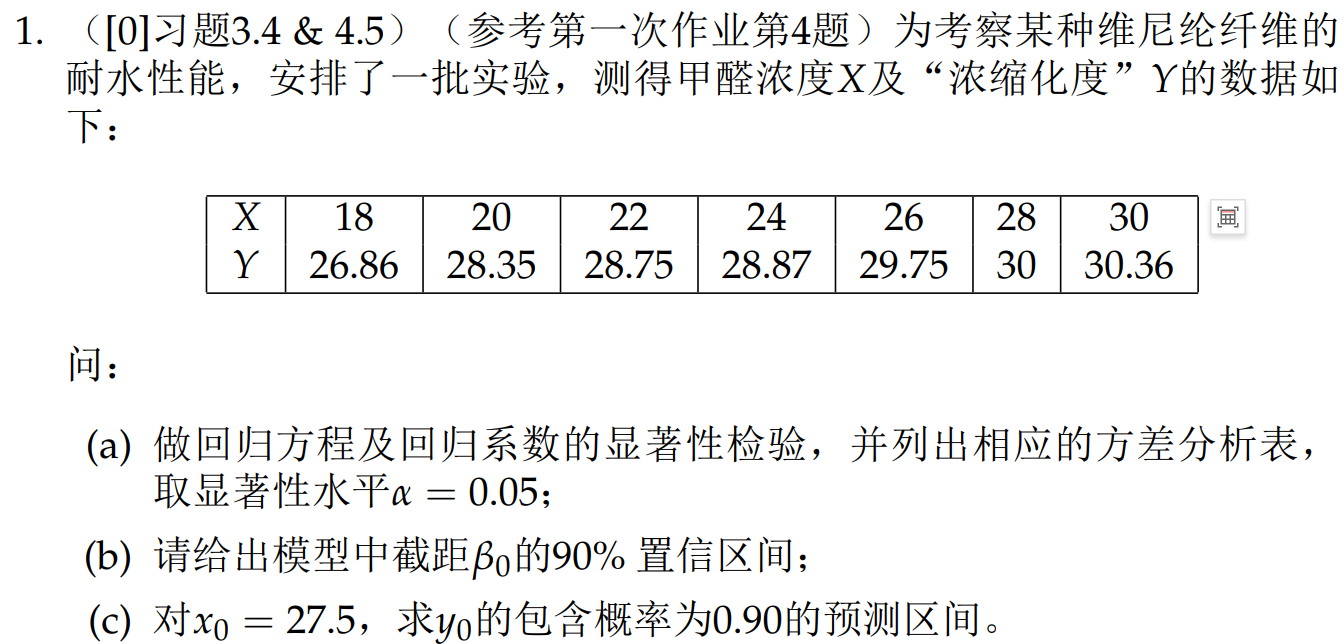
\includegraphics[width=30em]{image/hw5_1.png}
\end{figure}

\begin{proof}[\solutionname]
\end{proof}

(a) $\bar{x}=24$,$\bar{y}=28.99$,$SXX=112$,$SXY=29.6$,$SYY=8.49$

$\hat{\beta}_1 = \frac{SXY}{SXX} = 0.26$,$\hat{\beta}_0 = \bar{y} - \bar{x} \hat{\beta}_1 = 22.65$

$RSS = SYY-\frac{SXY^2}{SXX} = 0.67$,$SS_{reg} = SYY-RSS = 7.82$,$\hat{\sigma}^2 = \frac{RSS}{n-p} = 0.134$

$c_{00} = \frac{1}{n} + \frac{\bar{x}^2}{SXX} = 5.29$,$c_{11} = \frac{1}{SXX} = 0.0089$

回归系数的显著性检验:
$$
t_0 = \frac{\hat{\beta}_0}{\hat{\sigma} \sqrt{c_{00}}} = 26.91, \ t_1 = \frac{\hat{\beta}_1}{\hat{\sigma} \sqrt{c_{11}}} = 7.64
$$
临界值$t_5(0.025) = 2.57$,都拒绝原假设。

回归方程的显著性检验与相应的方差分析表:

\begin{center}
\begin{tabular}{|c|c|c|c|c|}
  \hline
  来源 & d.f. & SS & MS & F \\
  \hline
  X的回归 & 1 & 7.82 & 7.82 & 58.36 \\
  \hline
  残差 & 5 & 0.67 & 0.134 & {} \\
  \hline
  总的 & 6 & 8.49 & {} & {} \\
  \hline
\end{tabular}
\end{center}

临界值$F_{1,5}(0.05) = 6.61$,拒绝原假设。

(b) $\frac{\hat{\beta}_0-\beta_0}{\sigma \sqrt{c_{00}}} \sim N(0,1)$,$\frac{(n-p) \hat{\sigma}^2}{\sigma^2} \sim \chi^2_{n-p}$,故$\frac{\hat{\beta}_0-\beta_0}{\hat{\sigma} \sqrt{c_{00}}} \sim \mathit{t}_{n-p}$,可得$\hat{\beta}_0$的90\%置信区间
$$
\left[ \hat{\beta}_0-\mathit{t}_{n-p}(\frac{\alpha}{2})\hat{\sigma} \sqrt{c_{00}} , \hat{\beta}_0+\mathit{t}_{n-p}(\frac{\alpha}{2})\hat{\sigma} \sqrt{c_{00}} \right] = \left[ 20.95,24.34 \right]
$$

(c) 根据课件3.3节的公式,$y_0$的预测区间为
$$
\left[ \hat{y}_0-\hat{\sigma}\sqrt{1+d_0}\mathit{t}_{n-p}(\frac{\alpha}{2}),\hat{y}_0+\hat{\sigma}\sqrt{1+d_0}\mathit{t}_{n-p}(\frac{\alpha}{2}) \right]
$$
其中$\hat{y}_0=22.65+27.5\times0.26=29.92$,$d_0 = \frac{1}{n} + \frac{(x_0-\bar{x})^2}{SXX}=0.25$,则$y_0$的包含概率为0.90的预测区间为$\left[ 29.09,30.74 \right]$。


\newpage

\begin{homework}   
\end{homework}
\begin{figure}[!htbp]
    \centering
    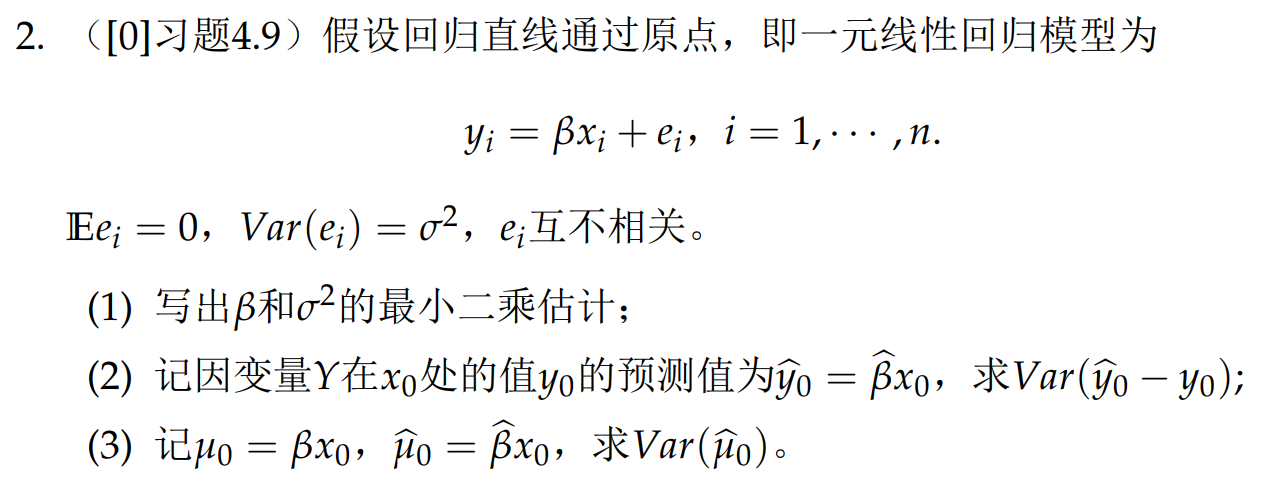
\includegraphics[width=30em]{image/hw5_2.png}
\end{figure}

\begin{proof}[\solutionname]
\end{proof}

(1) $\hat{\beta} = (X^T X)^{-1} X^T y = \frac{\sum_{i=1}^n x_i y_i}{\sum_{i=1}^n x_i^2}$,$\hat{\sigma}^2 = \frac{1}{n-1} RSS = \frac{1}{n-1} \left[ \sum_{i=1}^n y_i^2 - \frac{(\sum_{i=1}^n x_i y_i)^2}{\sum_{i=1}^n x_i^2} \right] $。

(2) $e_0$与$e_1,\cdots,e_n$互不相关,则$y_0$与$\hat{y}_0$互不相关,因此$\Var(\hat{y}_0-y_0) = \Var(\hat{y}_0) + \Var(y_0)$。其中$\Var(y_0)=\Var(e_0)=\sigma^2$,$\Var(\hat{y}_0)=x_0^2\Var(\hat{\beta})=x_0^2\sigma^2(X^T X)^{-1}=\frac{x_0^2 \sigma^2}{\sum_{i=1}^n x_i^2}$,故$\Var(\hat{y}_0-y_0)=\sigma^2(1+\frac{x_0^2}{\sum_{i=1}^n x_i^2})$。

(3) 由(2)的计算过程知,$\Var(\hat{\mu}_0)=\frac{x_0^2 \sigma^2}{\sum_{i=1}^n x_i^2}$。

\newpage

\begin{homework}   
\end{homework}
\begin{figure}[!htbp]
    \centering
    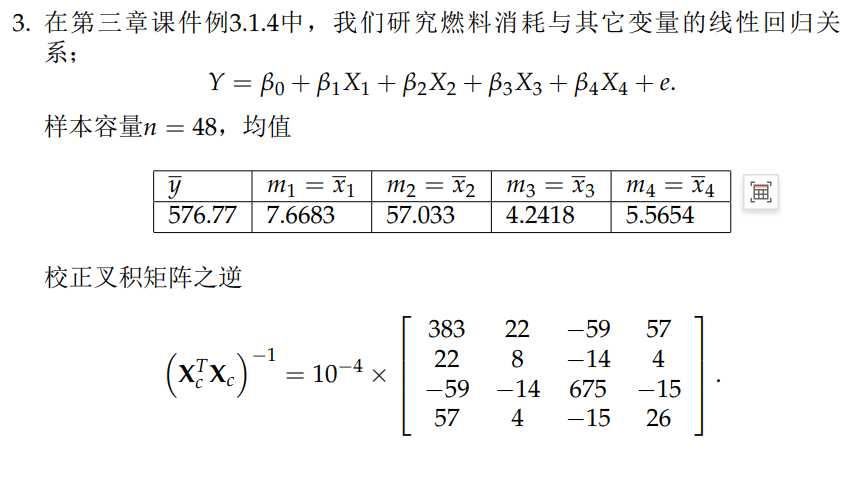
\includegraphics[width=25em]{image/hw5_3.png}
\end{figure}
\begin{figure}[!htbp]
    \centering
    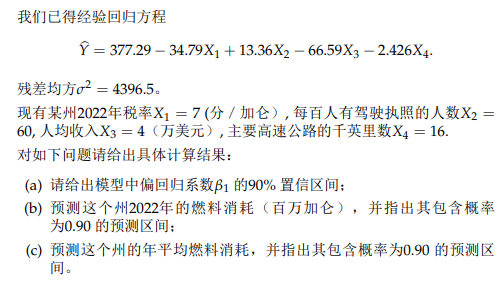
\includegraphics[width=25em]{image/hw5_3q.png}
\end{figure}

\begin{proof}[\solutionname]
\end{proof}

(a) 与第1题(b)问同理,$\beta_1$的置信区间为
$$
\left[ \hat{\beta}_1-\mathit{t}_{n-p}(\frac{\alpha}{2})\hat{\sigma} \sqrt{c_{11}} , \hat{\beta}_1+\mathit{t}_{n-p}(\frac{\alpha}{2})\hat{\sigma} \sqrt{c_{11}} \right]
$$
其中$\hat{\beta}_1=-34.79$,$\mathit{t}_{n-p}(\frac{\alpha}{2})=\mathit{t}_{43}(0.05)=1.68$,$\hat{\sigma}^2=4396.5$,$c_{11}=0.0383$,则偏回归系数$\beta_1$的90\%置信区间为$\left[ -56.60,-12.98 \right]$。

(b) 根据课件3.3节的公式,点预测区间为
$$
\left[ \hat{y}_0-\hat{\sigma}\sqrt{1+d_0}\mathit{t}_{n-p}(\frac{\alpha}{2}),\hat{y}_0+\hat{\sigma}\sqrt{1+d_0}\mathit{t}_{n-p}(\frac{\alpha}{2}) \right]
$$
其中$\hat{y}_0=377.29-34.79\cdot7+13.36\cdot60-66.59\cdot4-2.426\cdot16=630.184$,$d_0 = \frac{1}{n} + (x_0-m)^T (X_c^TX_c)^{-1} (x_0-m)=0.276$,则2022年燃料消耗的90\%预测区间为$\left[ 504.26,756.11 \right]$。

(c) 根据课件3.3节的公式,年平均燃料消耗的90\%预测区间为
$$
\left[ \hat{y}_0-\hat{\sigma}\sqrt{d_0}\mathit{t}_{n-p}(\frac{\alpha}{2}),\hat{y}_0+\hat{\sigma}\sqrt{d_0}\mathit{t}_{n-p}(\frac{\alpha}{2}) \right] = \left[ 571.60,688.77 \right]
$$


\newpage


\begin{homework}   
\end{homework}
\begin{figure}[!htbp]
    \centering
    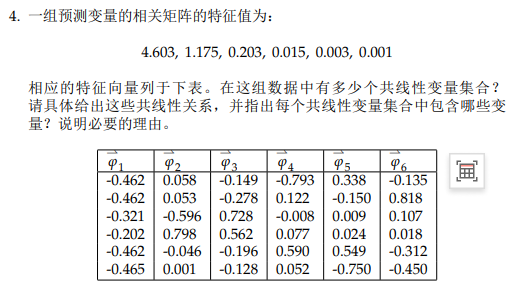
\includegraphics[width=30em]{image/hw5_4.png}
\end{figure}

\begin{proof}[\solutionname]
\end{proof}

相关矩阵的特征值$\lambda_5, \lambda_6 \approx 0$,因此这组数据中有两个共线性变量集合,具体的共线性关系分别是
$$
0.338 \frac{X_1 - m_1}{s_1} - 0.150 \frac{X_2 - m_2}{s_2} + 0.024 \frac{X_4 - m_4}{s_4} + 0.549 \frac{X_5 - m_5}{s_5} - 0.750 \frac{X_6 - m_6}{s_6} \approx 0
$$
包含变量$\left\{ X_1,X_2,X_4,X_5,X_6 \right\}$,与
$$
-0.135 \frac{X_1 - m_1}{s_1} + 0.818 \frac{X_2 - m_2}{s_2} + 0.107 \frac{X_3 - m_3}{s_3} + 0.018 \frac{X_4 - m_4}{s_4} - 0.312 \frac{X_5 - m_5}{s_5} - 0.450 \frac{X_6 - m_6}{s_6} \approx 0
$$
包含变量$\left\{ X_1,X_2,X_3,X_4,X_5,X_6 \right\}$。

\begin{note}
    我们约定数值$c \leq 0.01$时,认为$c \approx 0$。
\end{note}


\newpage


\begin{homework}   
\end{homework}
\textbf{题目修改:方差分析表中,“关于X2,X3的回归”中“平方”的值改为151.086.}
(因为由之后主成分形式的计算可知$SS_{reg} = \sum_{i=1}^{3} \lambda_i \hat{\alpha}_i^2 \sim=154 $)

题干略,题目如下
\begin{figure}[!htbp]
    \centering
    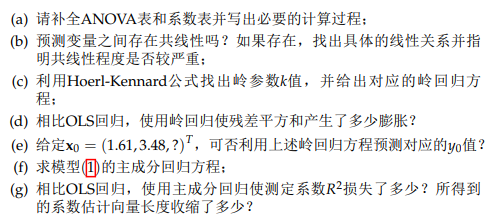
\includegraphics[width=30em]{image/hw5_5.png}
\end{figure}

\begin{proof}[\solutionname]
\end{proof}
\noindent (a)
\begin{align*}
    & d.f.^{2,3} = 2, \quad MS_{reg}^{2,3} = \frac{309.304}{2} = 154.652, \\
    & d.f.^1 = 1, \quad \widetilde{MS}_{reg}^1 = 2.7504, \\
    & d.f. = 60, \quad \hat{\sigma}^2 = \frac{122.640}{60} = 2.044, \\
    & t_0 = \frac{-1,230}{2.431} = -0.506, \\
    & F_1 = \frac{\widetilde{MS}_{reg}^1}{\hat{\sigma}^2} = 1.346, \\
    & t_1 = \sqrt{F_1} = 1.160, \quad \hat{\beta}_1 = 1.160 \cdot 0.783 = 0.908, \\
    & \hat{se}(\hat{\beta}_2) = \frac{1.032}{0.743} = 1.389, \\
    & \hat{\beta}_3 = 1.529 \cdot 0.260 = 0.398.
\end{align*}

\noindent (b) 相关系数矩阵的特征值$\lambda_3=0.01$,则存在共线性关系,条件数$k = \frac{1.93}{0.01}=193$,则共线性程度中等或较强。具体的共线性关系为
$$
0.514 \frac{X_1-2.45}{9.487} + 0.501 \frac{X_2-6.29}{5.220} - 0.696 \frac{X_3-3.96}{6.525} = 0
$$
可化简为$0.0542X_1 + 0.0960X_2 -0.1067X_3 = 0.3140$。

\noindent (c) 
\[\hat{\beta}_s = \hat{\beta}_c * s\footnote{这里$s = (s_1, s_2, s_3)$,乘法表示逐元素相乘。}=(8.61, 5.39, 2.6)^T, \quad \hat{\alpha} = \Phi ^T \hat{\beta}_s=(8.78, -2.14, 5.32)^T\]
由Hoerl-Kennard 公式,
\[\hat{k} = \dfrac{\hat{\sigma^2}}{\max_i \hat{\alpha}_i^2} = \dfrac{2.044}{8.78^2} = 0.0265, \quad \hat{\alpha}(\hat{k}) = (\Lambda + \hat{k} I)^{-1}\Lambda \hat{\alpha} = (8.66, -2.08, 1.46)^T\]
\[\hat{\beta_s}(\hat{k}) = \Phi \hat{\alpha}(k) = (6.53, 3.43, 5.2)^T, \quad \hat{\beta_c}(\hat{k}) = \hat{\beta_s}(\hat{k})/s = (0.688, 0.656, 0.797)^T\]
\[\Bar{y} = 1*(-1.23) + m^T\hat{\beta}_c = 9.06\]
对应方程
\[Y = 9.06 + 0.688(X_1 - 2.45) + 0.656(X_2 - 6.29) + 0.797(X_3 - 3.96)\]

\noindent (d) 由方差分析表$SYY = 309.304+2.7504+122.64 = 434.6944, \quad RSS = 122.64$。
对于岭回归方程
\[y = \alpha_0(k)\bm 1 + Z\alpha(k) + e\]
Claim:
\begin{align*}
    RSS(k) = RSS(0) +  k^2\sum_{i = 1}^{p-1}\dfrac{\lambda_i}{(\lambda_i + k)^2}\hat{\alpha}_i^2
\end{align*}
(证明如下
\begin{align*}
    RSS(k) &= ||y_c - Z\hat{\alpha}(k)||^2 = ||y_c - Z\hat{\alpha} + Z\hat{\alpha}-Z\hat{\alpha}(k)||^2 \\
    & = RSS(0) + 2(y_c - Z\hat{\alpha})^TZ(\hat{\alpha}-\hat{\alpha}(k))+ ||Z(\hat{\alpha}-\hat{\alpha}(k))||^2\\
\end{align*}
注意到交叉项为0(直接计算或利用OLS正交性)
\begin{align*}
    ||Z(\hat{\alpha}-\hat{\alpha}(k))||^2 &= (\hat{\alpha}-\hat{\alpha}(k))^T\Lambda (\hat{\alpha}-\hat{\alpha}(k)) \\
    &= (I - (\Lambda +kI)^{-1}\Lambda\hat{\alpha})^T\Lambda (I - (\Lambda +kI)^{-1}\Lambda\hat{\alpha})\\
    & = k^2 \hat{\alpha}^T(\Lambda + kI)^{-1}\Lambda (\Lambda + kI)^{-1} \hat{\alpha} \\
    & =  k^2\sum_{i = 1}^{p-1}\dfrac{\lambda_i}{(\lambda_i + k)^2}\hat{\alpha}_i^2
\end{align*})

故\[
RSS(\hat{k})- RSS(0) = \hat{k}^2\sum_{i = 1}^{p-1}\dfrac{\lambda_i}{(\lambda_i + \hat{k})^2}\hat{\alpha}_i^2 = 0.1794152\]
增长率$0.179/122.64 = 0.145\%$

\noindent (e) 由于我们已知模型变量中有较强的共线性关系,利用其先推测$X_3$取值。
\[0.0542X_1 + 0.096X_2 -0.1067X_3 = 0.3140 \Rightarrow x_{0,3} = 1.006 \]
代入岭回归方程
\[\Tilde{y_0} = 9.06 + 0.688(x_{0,1} - 2.45) + 0.656(x_{0,2} - 6.29) + 0.797(x_{0,3} - 3.96) = 4.2859\]

\noindent (f) 第三特征值约为0,前两主成分的累计方差贡献率为$\dfrac{1.93+1.06}{3} = 0.99$,故取前两主成分(r = 2)。
\[\hat{\beta}_{s,P} = \Phi_1 \hat{\alpha}_1 = \begin{bmatrix}
    0.5 & -0.697\\
    0.484 & 0.717 \\
    0.718 & 0.002\\
\end{bmatrix}\begin{bmatrix}
    8.78\\
    -2.14\\
\end{bmatrix} = \begin{bmatrix}
    5.8785\\
    2.7172\\
    6.2990\\
\end{bmatrix}\quad \hat{\beta}_{c,P} = \hat{\beta}_{s, P}/ s = \begin{bmatrix}
    0.62\\
    0.521\\
    0.965\\
\end{bmatrix}
\]
因此主成分(r = 2)回归方程为:
\[Y = 9.06 + 0.62(X_1 - 2.45) + 0.521(X_2 - 6.29) + 0.965(X_3 - 3.96)\]

\noindent (g) 
Claim:
主成分估计$RSS_P$(r个主成分)与原$RSS$关系为
\[RSS_P = RSS + \sum_{i = r+1}^{p-1}\lambda_i \hat{\alpha}_i^2\]
(证明:
\begin{align*}
    RSS_P &= ||y_c - Z\hat{\alpha}_P ||^2 = ||y_c -Z\hat{\alpha} +Z\hat{\alpha} - Z\hat{\alpha}_P||^2\\
    & = RSS + ||Z(\hat{\alpha}- \hat{\alpha}_P)||^2\\
    & = RSS + ||Z_2\hat{\alpha}_2||^2\\
    & = RSS + \sum_{i = r+1}^{p-1}\lambda_i \hat{\alpha}_i^2
\end{align*})

利用\textbf{最原始定义}$R^2 = 1- \dfrac{RSS}{SYY}$,
\[R^2 - R_P^2 = \dfrac{RSS_P - RSS}{SYY} = \dfrac{0.2829311}{434.6944}=0.00065 \]
\[||\hat{\beta}_{c,P}|| = 1.259715, \quad ||\hat{\beta}_c|| = 1.431046, \quad ||\hat{\beta}_c||- ||\hat{\beta}_{c,P}|| = 0.171331 \]

\begin{note}
    (1) (c)问中最后的回归方程也可以进一步化简为\[Y = 0.0882 + 0.688X_1+0.656X_2+0.797X_3\]进而$\hat{\beta_0}(\hat{k}) = 0.0882$

    \noindent(2)注意在\textbf{岭回归(k>0)}中,\textbf{没有} $SYY = RSS_{reg} + RSS$。且要注意$R^2 = 1- \dfrac{RSS}{SYY}$才是最原始的定义。这是因为在一些压缩估计中,OLS“投影”的性质被破坏,也就失去了等式背后的“直角三角形”。
    
  \noindent  (3) (d)问中,我们可以也计算下$SS_{reg}$玩玩。\[SS^{ridge\_k}_{reg} = \hat{\alpha}(k)^T\Lambda \hat{\alpha}(k) = \hat{\alpha}^T\Lambda(\Lambda + kI)^{-1}\Lambda (\Lambda + kI)^{-1}\Lambda \hat{\alpha} = \sum_{i=1}^{p-1} \dfrac{\lambda_i^3}{(\lambda_i + k)^2}\hat{\alpha}_i^2 \]
  又有
  \[RSS(k) = RSS(0) + k^2\sum_{i = 1}^{p-1}\dfrac{\lambda_i}{(\lambda_i + k)^2}\hat{\alpha}_i^2, \quad RSS(0) = SYY - SS_{reg} (0) = SYY-\sum_{i = 1}^{p-1}\lambda_i\hat{\alpha}_i^2\]
  得
  \[RSS(k) = SYY-\sum_{i = 1}^{p-1}\lambda_i\hat{\alpha}_i^2+k^2\sum_{i = 1}^{p-1}\dfrac{\lambda_i}{(\lambda_i + k)^2}\hat{\alpha}_i^2=SYY - \sum_{i = 1}^{p-1}\dfrac{\lambda_i^2(2k+\lambda_i)}{(\lambda_i + k)^2}\hat{\alpha}_i^2\]
  因此随着$k$的增大,$SS_{reg}$减小。由$RSS'(k) = \sum_{i = 1}^{p-1} \dfrac{2k\lambda_i^2}{(\lambda_i + k)^3}\hat{\alpha}_i^2 \ge 0$,$RSS(k)$随$k$单增。当k趋于无穷时,$SS_{reg}$趋于0且$RSS$趋于$SYY$。此时相当于对系数大小加的惩罚系数过大,致使所有系数为0。对应到$\hat{\beta}(k)$MSE的方差偏差分解,即偏差非常大,方差为0(因为常数的方差为0)。类比思考Lasso估计。

  \noindent (4)同理计算主成分估计的$SS_{reg}$。
  \[SS_{reg} = ||Z1\hat{\alpha}_1||^2 = \sum_{i = 1}^r \lambda_i \hat{\alpha}_i^2\]
  这时候可以检验$SYY = SS_{reg} + RSS$是成立的。(几何上是因为Z为列正交阵,主成分估计取前r个分量,相当于往Z前r列空间投影)
\end{note}


\newpage

\begin{homework}   
\end{homework}
\begin{figure}[!htbp]
    \centering
    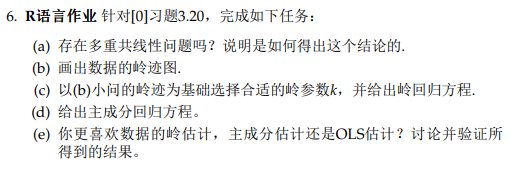
\includegraphics[width=30em]{image/hw5_6.png}
\end{figure}

\begin{note}
    主成分分析中,也可以考虑累计方差占比来选择最终主成分。
\end{note}


\end{document}